\section{Exploiting Callbacks}
Android framework provides a variety of callback functions for developers conducting their apps a particular responding after a specific event happens. Yet, abusing these callbacks would incur undesirable consequence as well.
\subsection{Motivating Example}

\begin{figure*}[t]
\centering
\scalebox{1}[0.8]{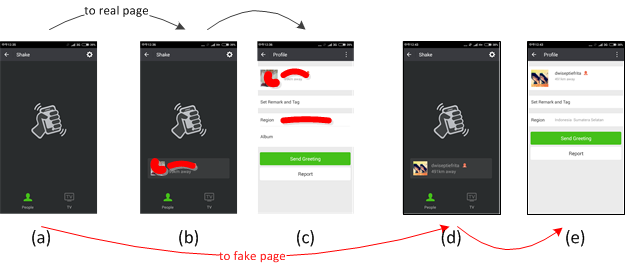
\includegraphics{pic1.png}}
\caption{\label{} Motivating example about the PEC threats. In (a), a user prepare to try the "Shake"; (b) shows a normal case that a real result popped up after shake; (c) presents the further information of such real page after user clicks the result; (d) shows the case that the shake action is perceived by an adversary app, which pop up a fake "result" page after it receives the shake action; (e) presents the further fake information crafted by attacker, which is used to induce user to convince it.}
\end{figure*}

We take the well-known app Wechat as a motivating example. Wechat is known as a popular IM(Instant Messenger) tool for users sharing information and connecting with each other. Of diverse functionalities it provides, "Shake" is rather welcomed, which enables users to randomly obtain an online chatting partner so long as slightly shaking the device several times.

Although harmony in surface, there exists potential crisis in the user shaking action which can be easily perceived by any other app through the {\color{red}SENSOR\_SERVICE}, a system service for managing inner device sensor. That is to say, only with the {\color{red}SystemSensorManager} object instantiation and the arrangement of shaking action size , an adversary app could clearly receive the same action event signal as Wechat. Further more, associating with the running status of Wechat through {\color{red}AMS(Activity Manager Service)}, adversary app could naturally make a judgement about the accurate time when the Wechat responding page would be popped up after user shaking. Although there exists an exception that user could shake the device in other page of "Wechat",the possibility of the exception's emergence is scarcely small in practice because user shakes device in such wide margin normally with intensive intention. {\color{red}Figure 1} shows how the "Shake" event is "stolen" by others. 

It seems that the PEC threats is easily ignored by developers and app markets. We see the callback time leakage severely because it offers a big change for attackers. A wily attacker could devise diverse attacks utilizing the PEC threats. For instants, attackers could deliberately construct a similar result page that links to a malicious third-party chatting tool, or even mimic a fake chatting page to pretend to chat with user for malicious purpose. We presents greater details about the attacks in section **.

\subsection{PEC Model} 

In order to clearly illustrate the callback threats, we view the threats process as a kind of callback state model. Each PEC within a installed app can be described as (S,D,E,C), where "S" denotes current state of app, which can be observed by other apps; "D" denotes the display-sink contained by the callback function; "E" denotes the event that invokes executing of the callback function; "C" denotes the proper control flow conditional values towards the "F".

\paragraph{Component-state}

(s belongs to S)The component-state refers to if the components of an app are running, which provides basic materials to PEC. Similar to the Event, the component-state here also needs to be exposed to other apps.

Before {\color{red}Android 5.0} emerging, the execution state of component like Activity and Service can be easily observed by the {\color{red}getRunningTasks API in ActivityManager object}. A more detailed observation needs to request the "GET\_TASK" permission, which could somehow attract the attention of most of normal users. However, Android starts to constraint the usage of such permission request and the usage of related API from recent {\color{red}Android 5.0+} for the security consideration. The getRunningTasks and even getRunningAppProcess(the API for get all the running process in the device) are now deprecated and only return developer's own application process. {\color{red}A substitute solution is to request new "PACKAGE\_USAGE\_STATS" permission, and to disable warning that permission is system level and will not be granted to third-party apps. Again, this approach needs extra permission request. } A decent solving method to get the foreground running app without any permission request is introduced in  \cite{getforeground} through reading the /proc file where Linux preserves all its process information. For all, obtaining the foreground app is entirely a completable task in common Android system version. 

Another good news is that the usage of  "getRunningServices" are still available in the newest version and need not request any extra permission. Thus, we can judge if a typical service is running through the "getRunningServices" API without any permission request. 

In addition, statically-registered BroadcastReceiver always in the receiving state when the app is running, so its component-state is also easy to ensure. On the other side, the component-state of dynamically-registered BroadcastReceiver follows the running state of its host component, e.g., activity and service, and the method where it is registered.


\paragraph{Display-sink}

(d belongs to D)Display-sink is based on the conception of leakage detection, which refers to a set of label functions that can expose data or information to outside. However, different from traditional conception, Display-sink here specifically refers to state output that could be perceived by users rather than information leakage, including UI page, dialog or notification, etc.

As to the Display-sink, only those output vectors which can be leveraged by attackers are considered. Most of which are related to UI activity, causing the UI is designed as the main channel to interact with users. Some of the UI vectors are mentioned in recent research\cite{bianchi2015app}(e.g., startActivity API, Toast message), yet we also collect some other UI related vectors, e.g., AlertDialog.Builder API, NotificationManager API. Generally, both of Dialog and Notification need response from users(e.g., click) and then engage corresponding reaction functionalities, which offers chance for attackers to interfere the users behaviours, which is insecure.

\textbf{Dialog}
Generally speaking, it goes against Android design and UI guidelines that directly launching a Dialog from Service or BroadcastReceiver. Therefore, if Dialog is roughly created from a Service or BroadcastReceiver, there would pop up an error report causing Dialog is implemented relying on a particular Activity. However, it is pretty work that setting a system alert Dialog with the "SYSTEM\_ALERT\_WINDOW" permission grant. This kind of Dialog has global feature that can be invoked by a Service or a system event rather than an Activity. 

\textbf{Toast}
In common case, the Toast is also constructed based on an existing Activity rather than Service or BroadcastReceiver. The reason of that is one of Toast.makeToast parameters refers to the main UI context the one belongs to. Therefore, directly popping up from Service or BroadcastReceiver would not work causing the UI context is erroneously referred. However, a common-used tool class "Handler" can be used to insert the self-defined thread message into the main thread queue, so that the main thread UI context can be obtained by the Toast. Therefore, Toast can be launched not only in Activity but also in Service and BroadcastReceiver.

\textbf{StartActivity}
The startActivity is known to be invoked by all the three components. However, some Activity is set self-defined permission to improve the security protection. For those low risk "protectionLevel", namely "normal" and "dangerous", we can still apply corresponding self-defined permission to access the target components. Nevertheless, for those high risk level, namely "signature" and "signatureOrSystem", currently there is no any effect way to access the target components by a third party app.

\textbf{Notification}
The Notification can be launched by all the three components as well. Compare to Dialog and Toast, Notification is more likely used in service for notify the task progress or updated information. 



Besides UI sink, some non-UI vectors are also contained, e.g., audio, vibrate related API, sendBroadcast, startService. Similar to UI related vectors, audio and vibrate related API also engage information output although as different information forms("voice and vibration"). The "sendBroadcast" and "startService" is able to lead new callbacks, which threatens the targeted app in a iterative way. Additionally, implicit intent loaded by "sendBroadcast" and "startService" also can be leveraged by attackers.

\paragraph{Event}

(e belongs to E) The event here refers to the public event since non-public one can hardly be exploited by other apps. As mentioned in section **, public events lie in all the three event categories(life-cycle, user-driven and system).

\paragraph{Control Flow}

(C)Control Flow is a collection of conditional values over the path from a typical State to a Display-sink. In theory, as for a callback threat vulnerable app, the "C" needs to guarantee an observable and feasible path that can reach the Display-sink. However, the "C" that strictly conforms above definition rarely emerges in real apps, so that we adopt a more flexible mechanism in practice which will be introduced in next section.  

Attackers need to find a feasible path from the State to the Display-sink within the given operable source code of a target app. For judging the existing of such path, we first collect the condition set of the paths to the Display-sink. Then a signal used to refer to if it is visible for each value, event and function emerging in the condition set is created. To describe more clearly, we denote the following concepts:

1. c: the condition value of each branch.

2. CS: the condition set collected from a program control flow path.

3. cv(a) : the condition value of variable a and a = variable | function | event

4. s(a): the signal value of variable a and a = variable | function | event, whose type is boolean.

s(a) represents if the variable a can be observed by components from other apps. s(a) = true represents yes, s(a) = false represents no.

5. CS = $\cap$ ( cv(a) \& s(a) ) = ($\cap$(c)) \& ( $\cap$ s(a))

Above equation means the value of condition set of a particular path consists of two parts, 1. the value of each variable; 2. the signal value of it. A feasible path needs not only has a solvable condition set, but also observable for each variable. However, practically we normally use the second equation to compute the feasibility of a target path. First, computing out if it is feasible for each branch ; then , considering if it is able to be observed for each variable with the branch condition.

A traditional technique for above computation is symbolic execution. However, it needs unacceptable overhead in practice. {\color {red} To the end, we using an improved SMT approach to solve the constraint conditions.} Normally there should be feasible from source to sink in a target app, otherwise there exists a designation shortage with in the target app. Under this prerequisite, we only need to consider s(a), namely if all the variables are observable. 



%\begin{figure}[t]
%\centering
%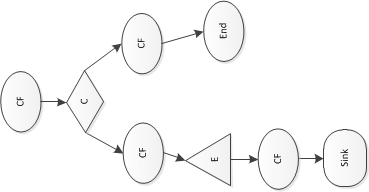
\includegraphics[width = 3.0in]{control-flow.png}
%\caption{\label{}control-flow}
%\end{figure}
%
%\begin{figure}
%\centering
%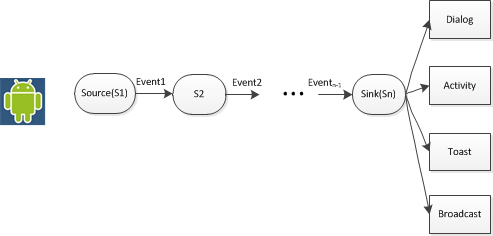
\includegraphics[width = 3.0in]{principle0.png}
%\caption{\label{} principle0}
%\end{figure}
%
%\begin{figure}
%\centering
%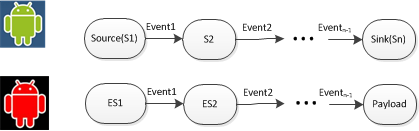
\includegraphics[width = 3.0in]{principle.png}
%\caption{\label{}principle1}
%\end{figure}



\begin{table*}[htbp]
\centering
 \caption{\label{tab:test} Typical vectors of PEC}
 %\begin{tabular}{lcll}
 \begin{tabularx}{\linewidth}{XXXX}

  \toprule
  State & Display-sink & Event & Control Flow \\
  \midrule
 1.Activity running state(Launching page) & 1.startActivity & 1.Broadcast from system: \{Intent.ACTION\_BATTERY\_LOW\} & 1.branch or cycle condition analysis \\
  2. Service running state &2. Toast message & 2.Implicit Intent\& pendingIntent & 2.method invocation analysis\\
     & 3.AlertDialog. Builder & 3.ServiceManager(need not permission grant): { sensorManager, memoryManager }\\
     & 4.sendBroadcast (intent)& 4.ServiceManager(need permission grant): { batteryManager }\\     
     & 5.AudioManager API & \\
     & 6.VibrateManager API & \\
     & 7.NotificationManager API & \\
     
  \bottomrule
 \end{tabularx}
\end{table*}



{\color{red}Table 2} lists the main vulnerability vectors with the callback threats. 
